\documentclass[a4paper,10pt]{article}
\usepackage[utf8]{inputenc}
\usepackage{graphicx}

%opening
\title{User's Guide for TDATools Package}
\author{}

\begin{document}

\maketitle

\begin{abstract}
words
\end{abstract}

\section{Getting Started}


\paragraph{System Requirements}

The TDATools package should work on all common platforms, and has been tested on Windows, Mac, and several Linux variants.

Obviously, you will need MATLAB on your machine.
The package has been tested on Matlab 2013b and 2014a, with all toolboxes installed.  Various components use commands available only in certain toolboxes (for example, the mapping toolbox is required for rca1mfscm).  We provide no guarantee that all tools will work on earlier versions of Matlab.  We strongly recommend that you use this package on a complete installation of Matlab, including all toolboxes.  
If you encounter an error running one of the commands, and your script calls are syntactically correct, please email Rann Bar-On (rann@math.duke.edu) for help.  We would be glad to let you know what toolbox may be missing so that you may install it, and/or and possibly work with you to provide an alternative method, with the caveat that the latter may decrease performance.

Although all of the commands in this package are written in MATLAB, quite a few of them (LSD.m and everything with the prefix rca) require interaction with the underlying
Java code in bin/tda.jar.
Facilitiating this on a particular computer or
operating system requires the availability of a Java virtual machine (JVM). The code has been written
to comply with Java 2, using the 1.6 or later release of the Java SDK.

\paragraph{Installation}

There are two main methods for obtaining the TDATools package, either via downloading a zip of the latest stable version from the website or by cloning 
the most recent version from our git repository.





\paragraph{Setting up MATLAB to run TDATools}

Follow these steps to get the TDATools package running in your MATLAB session.
Note that you must do this each time you start a new MATLAB session, assuming you want
to use the TDATools package during that session.

\begin{enumerate}
   \item Either run MATLAB in the TDA package directory, or make it the active directory in an already-running MATLAB session.  This directory contains the \textbf{init.m} file.
   \item At the MATLAB command prompt, execute the command $$>> \mbox{init}$$  This will set up your environment.\\
   \item Check that you now have a variable called TLDIR. This is a directory path which ends in tda/.
\end{enumerate}

That should be that, and you are now ready to start computing.





\section{Computing Persistence Diagrams}

The directory /src/MATLAB/topology contains all the .m files needed for computing persistence diagrams in various
ways. Here we go over each command in turn, first by just explaining the syntax and then by directing you to compute
some examples. The most basic command, involving Rips filtration on point clouds, is explained first, and
we then move to more exotic variants.
Note that the input and output files that we refer to can be found in /examples/Testing.

\subsection{Rips filtrations on point clouds.}

Let $X$ be a point cloud in Euclidean space.
The command rca1pc computes the persistence diagrams, in dimensions zero and one, for the Rips filtration built off of $X$.
Note that this command implements the Rips-Collapse algorithm (see arxiv paper), which returns the exact diagrams in time far
faster than the standard Rips algorithm.

Specifically, the command $$>> \mbox{[I J] = rca1pc(X,distanceBoundOnEdges)};$$
produces two diagrams. 
$I$ is the $1$-dim persistence diagram for the Rips filtration on $X$, run up to Rips-threshold distanceBoundonEdges,
and $J$ is the $0$-dim diagram for the same filtration.
The diagrams are returned as $M \times 2$ arrays, where $M$ is the number of dots in the diagram,
and the two columns store birth and death values.
The input point cloud $X$ must come as a $N \times D$ array, where $N = |X|$, and $D$ is dimension of the Euclidean space.
The input distanceBoundOnEdges is just a real number.

\paragraph{Simple example.}

To test out this command, type
$$ >> \mbox{X = load('/examples/Testing/Diamond.txt');}$$
at the command line.
If you plot $X$, you will see that is just a set of four points taken from the corners of a diamond in the plane.
Now we compute
$$ >> \mbox {[I J] = rca1pc(X,3);}$$
and compare $I$ and $J$ to the output stored in /examples/Testing/Diamondonediagram.txt and /examples/Testing/Diamondzerodiagram.txt, respectively.
Assuming all has gone well, $I$ should store one one-cycle, and $J$ should store four components, with one being immortal
and the other three all dying at the same time.

Now try running rca1pc again on this point cloud, but with a distance bound of $1.5$. Does your output make sense?

\paragraph{Larger example.}

Now we compute the persistent homology of a large number of points sampled from a swiss roll.
First, type
$$ >> \mbox{Y = load('/examples/Testing/SwissRollSample.txt');}$$
at a command prompt. To plot $Y$, use the plot3 command:
$$ >> \mbox{plot3(Y(:,1),Y(:,2),Y(:,3));}$$
after rotating correctly you will see the swiss roll shape.

Now we compute
$$ >> \mbox {[K L] = rca1pc(Y,20);}$$
here $20$ is around the diameter of the point cloud.
Check $K$ against /examples/Testing/SwissRollonediagram.txt to verify output if you like.
Note that the $1$-dim persistence diagram $K$ has only one dot of ``large'' persistence, which makes sense.

\subsection{Rips Filtration on 'Distance Matrices'}

If you want to compute a Rips filtration using a different metric, then you just use the rca1dm command
in the following form
$$ >> \mbox {[I J] = rca1dm(D,distanceBoundonEdges);}$$
Here $D$ is a square matrix which stores the pairwise distances between the points in your point cloud,
and all other inputs and outputs are as in the description of rca1pc.

\paragraph{Example.}

As a silly check that this command does what it says it does, we take $Y$ to be the swiss roll sample
from above, and compute
$$>> \mbox{D = squareform(pdist(Y));}$$
That is, we let $D$ be the Euclidean distance matrix for $Y$.
Then we compute
$$ >> \mbox {[I J] = rca1dm(D,20);}$$
and note that the diagrams are identical to before.

\paragraph{Local homology.}

If you examine the code for rca1dm, you notice that there is no requirement that $D$ encode an actual metric.
Similarly, the defintion of a Rips filtration does not demand a metric.
All that is needed for $D$ is symmetry ($D(i,j) = D(j,i))$ and 
the fact that vertices have to come before their incident edges ($D(i,i) \leq D(i,j)$).
This flexibility proves useful in the comptation of local homology via LSD.m and then rca1dm.m, as we now describe.

First, type
$$ >> \mbox{X = load('/examples/Testing/CrossSample.txt');}$$
This is a set of points sampled from a cross in the plane, as you can verify by plotting.
We will now compute a good approximation (see arXiv paper) to the persistent local homology
diagram of $X$, with center point the origin, and radius of $0.3$.
To do this, we first compute the local spherical distance matrix:
$$ >> \mbox{D = LSD(X,[0 0], 0.3);}$$
As outlined in the arXiv paper, the $ij$-th entry of $D$ now stores the smallest $\alpha$ value
such that $B_{\alpha}(x_i) \cap B_{\alpha}(x_j) \cap \partial B_{0.3}(z) \neq \emptyset.$
We then feed $D$ to rca1dm, with the radius as distance bound, to finish the computation:
$$  >> \mbox{[I J] = rca1dm(D,0.3);}$$
Compare $J$ to the output stored in /examples/Testing/CrossZeroDiagram.txt; you should see four components of early birth, one with infinite lifetime.

\paragraph{Monotonic functions on simplicial complexes.}

The observation above about the minimal requirements on $D$ allows one to be quite flexible in using Rips methodology on a variety of filtrations.
For example, consider the simplicial complex $K$ shown in Figure \ref{fig:c}.
Recall that a monotonic simplex-constant function $f$ on $K$ is a series
of numbers $f(\sigma)$, one for each simplex $\sigma \in K$, subject to the requirment
that $f(\tau) \leq f(\sigma)$ whenever $\tau$ is a face of $\sigma$.
Such a function results in a filtration of $K$ by sublevel sets of $f$, and thus persistence diagrams, in the usual way.

Our package permits the computation of these diagrams, subject to an additional restriction on $f$; namely,
the $f$-value on a simplex $\sigma$ of dimension two or greater must simply be the maximum $f$-value on any of the edges contained in
$\sigma$.
If $f$ obeys this restriction, then we can produce a matrix $D$ which encodes the values of $f$, as follows.
\begin{figure}
 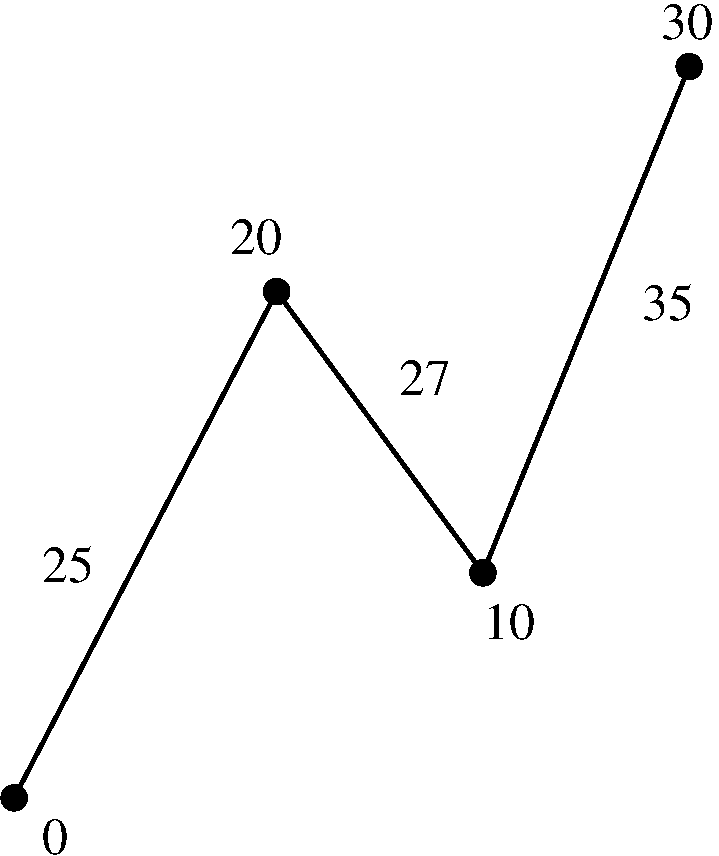
\includegraphics[scale=0.2]{complex}
\caption{A simplicial complex along with a simplex-constant monotonic function.}
\label{fig:c}
\end{figure}
We set $D[i,i]$ to be $f(v_i)$ and $D[i,j]$ to be the $f$-value of the edge connecting $v_i$ and $v_j$; if
$v_i$ and $v_j$ are not adjacent in $K$, then set $D[i,j]$ to infinity.
Feeding $D$ to rca1dm will then produce the persistence diagrams for this filtration.

However, doing this requires that you first create an $N \times N$ matrix $D$ where $N$ is the number of vertices in $K$, and
that will require too much memory for large complexes.
So we have included a different command, rca1mfscm, which allows one to get around this.
Specifically, you create a matrix $(N + M) \times 3$ matrix $S$, where $M$ is the number of edges.
$S$ must contain a row of the form $(i,i,f(i))$ for each vertex $v_i$, and a row of the form
$(i,j, f(i,j))$ for each edge between $v_i$ and $v_j$.
To create $S$ in our example, type
$$ >> \mbox{S = [0,0,0;1,1,10;2,2,20;3,3,30;0,2,25;1,2,27;1,3,35];}$$
Then feed $S$ to rca1mfscm with the command
$$ >> \mbox{[I J] = rca1mfscm(S,36);}$$
where we have chosen the distance bound to be larger than the maximum $f$-value.
In this example, $J$ will store the only interesting information.

Please read the comments on rca1mfscm.m for further discussion of this idea.

\subsection{Real-valued functions on intervals.}

We have also included a different command, MorseFiltration.m, that computes the 0-dim persistence diagram for the lower-star filtration
associated to a function based on sample values along an interval.
This code is optimized to be extremely fast for precisely this simple situation, and can generally handle far more input points than the commands above.

The basic command is
$$ >> \mbox{D = morseFiltration(f,aug,skew);}$$
The output, $D$, stores the persistence diagram as a many-by-2 array.
Here $f$ is a $1 \times N$ array, representing the values of $f$ sampled at $N$ incremented points along an interval.
The other two outputs are Boolean. Aug (default = false) indicated whether dots of persistence zero should be output,
and skew (default = false) indicates whether $D$ should store birth-lifetime instead of birth-death.

\paragraph{Example.}

Load the following input:

$$ >> \mbox{W = load('/examples/Testing/HarmonicPointSample.txt');}$$
which consists of $1000$ points sampled over $\frac54$ periods of a harmonic, as can be verified by plotting.
We now extract the second column of this array and feed it to the persistence code, as follows:
$$ >> \mbox{D = morseFiltration(W(:,2),false,false);}$$
Check $D$ against the ouptut stored in /examples/Testing/HarmonicZeroDiagram.txt.
















\end{document}
